\section{System-level Optimization}\label{section:system}

The majority of fuel cycle analysis effort involves users running single
simulations defined primarily by the deployment history of various facilities
over time.  In some cases, users may manually alter those deployment histories
to meet some objective, iterating until they find the best possible outcome.
In fewer instances, that iteration has been automated to seek optimal
solutions \cite{hays}.  By modeling discrete facilities over 1 month time
steps, \Cyclus{} offers many degrees of freedom for defining the deployment
history of its facilities, underscoring the value in an automated optimization
system.

This task focuses on the design, implementation and testing of a system that
uses \Cyclus{} to find optimal deployment histories within the bounds of
specific fuel cycle scenarios.  The first section defines a reference fuel
cycle scenario to be used when developing a system for fuel cycle
optimization.  The following section discusses the development of the basic
optimization system, including the choice of optimization algorithm and the
structure of the decision space.

This capability was then extended to seek an optimum deployment strategy under
the possibility of disruption of the fuel cycle at some future time.  The
methodology employed for this work used the same optimization algorithm, but
added nested layers of optimization to identify a hedging strategy that
minimizes the impact of a disruption during the transition.

\subsection{Reference Problem Description}

The EG23 transition defined by the Fuel Cycle Options campaign provided a
convenient problem for studying the optimization of fuel cycle scenarios.
This scenario starts with 100 \gls{LWR}s and follows an exponential growth of
  1\% per year for 200 years, while transitioning to a fuel cycle based
  entirely on \gls{SFR}s.  Plutonium from the separations of \gls{LWR} fuel is
  used to start the \gls{SFR} fleet, transitioning to recycling of their own
  fuel in the long term.  The deployment history of \gls{LWR} separations
  capacity is fixed, and reactor deployment history is to be optimized.  The
  goal is to complete the transition, defined by the decommissioning of the
  last \gls{LWR}, as quickly as possible.  More details of this transition are
  available in \cite{rwc_fff}.


  
\subsection{Black Box Optimization}

\subsubsection{Requirements and Algorithm Options}
Using a fuel cycle simulator as part of an optimization objective is a
challenging problem for several reasons:

\begin{itemize}
\item The objective function is generally not a linear function of input
  parameters.
\item No derivative information for the objective is available.
\item The objective function may be discontinuous.
\item Input variables to the objective function may be discrete.
\item The input parameter space could be large necessitating constraints
  for reasonable performance.
\item The objective function may be stochastic - i.e. different runs with
  the same inputs may produce different outputs.
\item The objective function is expensive to evaluate - seconds to minutes
  for a single iteration.
\end{itemize}

This kind of problem is often referred to as black-box optimization. Another
challenge is desirability of the optimization process to be effective over
many different simulation scenarios. There is no single, well-defined
objective to be optimized.

There are several classes of algorithms for addressing block-box optimization
of this nature:
\begin{itemize}
\item \textbf{Pattern Search} algorithms expand and contract their search over
  the decision space, with convergence governed by the rates of expansion and
  contraction.
\item \textbf{Swarm} algorithms follow the trajectories of a set of search
  points through the decision space, with the velocities of those points
  determined by the location and magnitude of the objective function at each
  evaluation.
\item \textbf{Evolutionary} algorithms evaluate the objective function across
  a population of points sampled from the decision space, and then look at
  ``genetic'' combinations of the best available points to identify better
  possible points.  Mutations can be used to modify the search process.
\item \textbf{Surrogate} algorithms form an approximate model of the objective
  function over the decision space, often of a form that can be optimized with
  algorithms that rely on information note available from the black-box
  approach.
\end{itemize}

In order to test these algorithms with the reference EG23 problem, it is
necessary to define the decision space and objective function.

\subsubsection{Decision Space Formulation}

Conceptually, the decision space is defined by the number of reactors of each
variety being deployed at each time step, with the total capacity constrained
to match the total electricity growth rate.  A naive implementation based on
this conceptual problem results in unbounded decision variables bounded by
explicit constraints.  Many black-box algorithms are challenged by such a
decision space, resulting in evaluations of infeasible solutions (those
outside the constraint) that are then penalized in the evaluation of the
objective function because of they are outside the constraint.  It is
therefore preferable to develop a formulation with a bounded decision space,
in which the constraints are represented by the bounds of the decision space.

The decision space for one such formulation is defined by the fraction of
capacity additions at each time step that will composed of each reactor type.
Each decision variable is then bounded on the interval $[0,1]$.  Furthermore,
by selecting the fraction of each reactor type in succession, and updating the
bounds for the next reactor type after each selection, the entire search space
is accessible without violating the constraint.

These fractions can be converted to the number of reactors as shown in
Equation \ref{eqn:tranform-reactors}.

\begin{equation}
    N(t, r) =
    \begin{cases}
        floor\left(\frac{
            \mathlarger{V_{fac}(t,r) \cdot \left[P_{new}(t) - \sum\limits_{r'=1}^{r-1} N(t,r') \cdot C(r')\right]}
        }{\mathlarger{C(r)}} + 0.5\right) & : r > 0 \\
        floor\left(\frac{
                \mathlarger{P_{new}(t) - \sum\limits_{r'=1}^{r_{last}} N(t,r') \cdot C(r')}
        }{\mathlarger{C(r)}} + 0.5\right) & : r = 0
    \end{cases}
    \label{eqn:transform-reactors}
\end{equation}

$N(t, r)$ is the number of reactors of type $r$ to deploy at time $t$,
$floor(x)$ is the closest integer to $x$ that is less than or equal to $x$,
$V_{fac}(t,r)$ is the decision variable value for facility $r$ at time $t$,
$P_{new}(t)$ is new capacity to be deployed at time $t$, and $C(r)$ is the
power capacity for a single reactor of type $r$ (e.g. 1000 MWe). The
$N(t,r=0)$ deployments must be computed after all $N(t, r > 0)$ deployments.
Reactor type $r=0$ is used to deploy any remaining new power capacity that is
not satisfied by the other reactor types.

\subsubsection{Objective Function}

Many possible objective functions can be used to assess fuel cycle
transitions, and selecting objective functions is an area of stuy in its own
right (in addition to defining them with sufficient certainty to be useful).
The objective function was designed to drive toward a fast-reactor-only fuel
cycle as quickly as possible while simultaneously discouraging/penalizing
unfueled reactors.  Because fast reactors are fueled only with recycled
fissile material, it is possible for some deployment schedules to cause fast
reactors to idle without fuel.  The objective function used is shown in
Equation \ref{eqn:obj}.

\begin{equation}
    \label{eqn:obj}
    O_{sim} = \frac{\sum\limits_{t \in sim} E_{t,\;LWR}}{\sum\limits_{t \in sim} E_{t,\;tot}}
\end{equation}

$O_{sim}$ is the objective function value for an entire simulation,
$E_{t,\;LWR}$ is the energy produced by all \gls{LWR}s in time step $t$, and
$E_{t,\;tot}$ is the energy produced by all reactors in time step $t$.
Because the optimizer is trying to minimize the objective value, more
\gls{LWR}s results in a larger numerator (a worse objective value), and
unfueled fast reactors shrinks the denominator (also a worse value).  It is
notable that this objective function does not penalize unfueled reactors very
heavily relative to the penalty for \gls{LWR} energy.  This is intentional and
allows the optimization to explore potentially interesting trade-offs related
to expediting the transition.


\paragraph{Master-worker implementation}

As black box techniques, all of the optimization algorithm classes explored
here rely on a large number of independent evaluations of the objective
function.  After the optimization algorithm selects the set of decision
variables for each evaluation, an objective function evaluation consists of a
\Cyclus{} simulation followed by some post-processing of the results.
Depending on the algorithm there were $O(200)$ evalutions per iteration, with
$O(300)$ iterations, for a total of $O(60,000)$ evaluations.  

The optimization system for \Cyclus{} was developed using a master-worker
paradigm in a high-throughput computing environment.  For each iteration, the
optimization algorithm ``master'' would assign work, in the form of a
\Cyclus{} input file, to a set of independent ``workers'', each of which would
run \Cyclus{} and evaluate the objective function based on the output.  Such a
system is flexible to the number of available workers at any time, and mutiple
masters can share the same pool of workers.  Such a system allowed a thorough
exploration of the different algorithms, with over 700,000 \Cyclus{}
evaluations used for the final comparison.  Development and testing relied on
about 1 million additional \Cyclus{} evaluations, consuming about 30,000 CPU
hours over 7 days.

\subsubsection{Algorithm Selection and Sample Results}

A variety of open source libraries, each implementing algorithms in one or
more of the classes of optimization algorithms, were tested for their
performance using the reference problem described above.

The overhead and time involved in dispatching and running Cyclus simulations
is much larger than the time and computational resources required to run the
each optimizer itself. Because of this, the optimizers are compared by
primarily looking at the best objective function value achieved as a function
of the total number of objective function evaluations.  Table
\ref{tab:exp1-summary} summarizes the results for all runs done with each
optimizer.  Only a single run was performed with the DIRECT algorithm because
it is deterministic and multiple runs on the same problem will always give the
same result.  The optimizers are listed in order of performance/effectiveness
with PSwarm being the best performer and DIRECT being the least effective.

\begin{table}[h]
    \centering
    \begin{tabular}{ |r | c c c c| }
        \hline                       
                      & Run & \# evaluations & \# iterations & Best objective \\
        \hline                       
        PSwarm          & 1 & 60,046 & 356            & 0.1704 \\
        PSwarm          & 2 & 60,062 & 349            & 0.1670 \\
        PSwarm          & 3 & 60,153 & 349            & 0.1671 \\
        PSwarm-biannual & 3 & 62,022 & 368            & 0.1423 \\
        JEGA            & 1 & 28,029 & 246            & 0.1884 \\
        JEGA            & 2 & 59,203 & 518            & 0.1848 \\
        JEGA            & 3 & 26,821 & 236            & 0.1889 \\
        HOPSPACK        & 1 & 60,012 & $310^\text{*}$ & 0.2816 \\
        HOPSPACK        & 2 & 59,840 & $310^\text{*}$ & 0.2637 \\
        HOPSPACK        & 3 & 59,956 & $310^\text{*}$ & 0.2900 \\
        SCOLIB EA       & 1 & 60,048 & 402            & 0.4742 \\
        SCOLIB EA       & 2 & 60,048 & 402            & 0.4871 \\
        SCOLIB EA       & 3 & 60,048 & 402            & 0.4871 \\
        SCOLIB DIRECT   & 1 & 58,260 & 16             & 0.5531 \\
        \hline                       
    \end{tabular}
    \captionsetup{justification=centering}
    \caption[Experiment 1: summary of optimizer runs]{

        Experiment 1 summary results for all optimizer runs. The additional
        \emph{PSwarm-biannual} run is identical to the other PSwarm runs
        except it had bi-annual instead of annual deployments resulting in only 200 optimization variables. \\
        
        \hspace{\textwidth}
        
        * The HOPSPACK optimizer did not have well-defined iteration
        boundaries.

    }
    \label{tab:exp1-summary}
\end{table}


The PSwarm and JEGA solvers were the strongest performers, with PSwarm beating
out JEGA slightly in both convergence rate and best solution found.  The other
solvers performed unsatisfactorily.  Figure \ref{fig:exp1-converge} provides a
good picture for roughly evaluating how each optimizer performed with respect
to the following criteria:

\begin{enumerate}

    \item How good was the best objective value found?

    \item How quickly did the optimizer converge toward a good solution?

    \item How consistently does the optimizer perform on criteria 1 and 2 over
        multiple runs and/or problems?

\end{enumerate}

In addition to the runs for each optimizer described above, Table
\ref{tab:exp1-summary} and Figure \ref{fig:exp1-converge} contain data from
one additional run using the PSwarm optimizer with bi-annual deployments
instead of annual deployments.  More detailed discussion of each result is
available in \cite{rwc-dissertation}.  The PSwarm optimizer was selected as
the primary optimization algorithm for the \Cyclus optimization system.

\begin{figure}
    \centering
    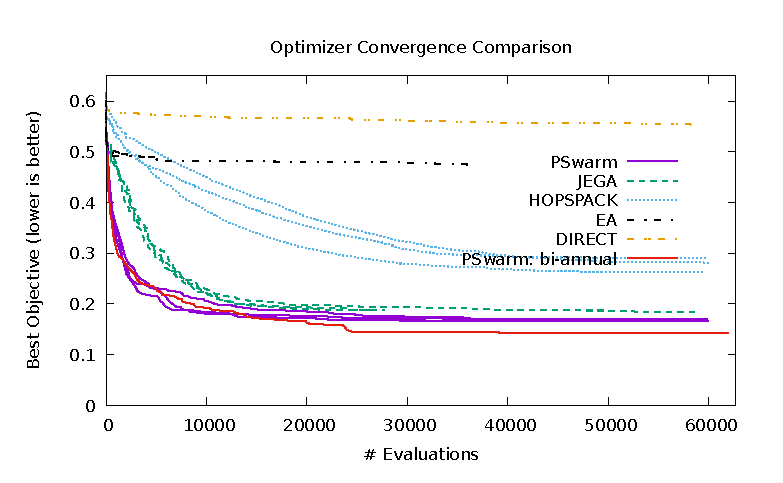
\includegraphics[width=1.0\textwidth]{converge.eps}
    \captionsetup{justification=centering}
    \caption[Experiment 1: optimizer convergence curves]{Objective value convergence curves for all optimizer runs.}
    \label{fig:exp1-converge}
\end{figure}

Figure \ref{fig:exp1-bestfoundpower} shows both the total power and LWR power
generated over time for the best deployment schedule found among all runs.
Figure \ref{fig:exp1-bestknownpower} shows both the total power and LWR power
generated over time for the best deployment schedule found by the PSwarm
optimizer using smaller $\pm5\%$ bounds instead of $\pm10\%$ bounds around the
growth curve. This deployment schedule results in an objective value of
$0.1557$.  This is noticeably better than the best result by other
400-variable optimizer runs which was $0.1671$ from the PSwarm optimizer.  The
larger 10\% power curve bounds effectively result in a solution space
containing $[\frac{\text{new range}}{\text{prev. range}}]^{n}$ times as many
possible solutions as the 5\% bounds where range refers to the difference
between upper and lower bounds and $n$ is the number of variables in the
problem. So doubling the size of the bounds for this 400-variable problem
results in a solution space with $2^{400}$ times as many possible solutions --
much larger than before.

\begin{figure}
    \centering
    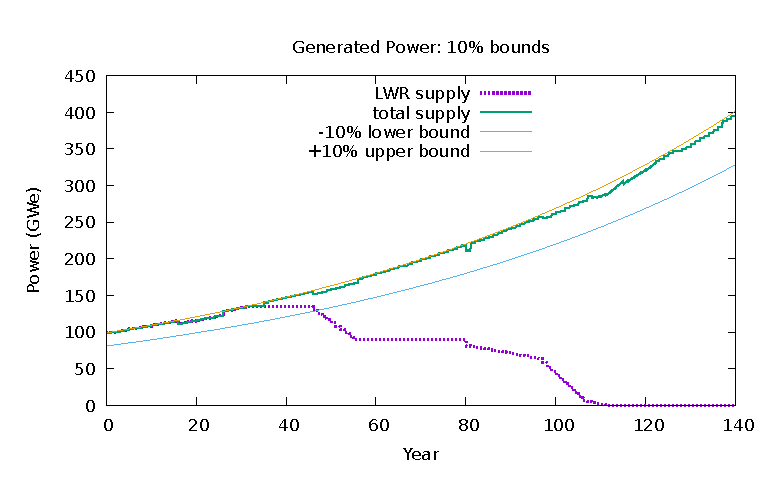
\includegraphics[width=1.0\textwidth]{best-found-power.eps}
    \caption[Power for best build schedule with $\pm10\%$ bounds]{ Both
      \gls{LWR} and total (\gls{SFR} and \gls{LWR}) generated power over time
      for the best deployment schedule found among all the primary
      optimization runs using the $\pm10\%$ bounds around the 1\% power growth
      curve and annual deployments.  }

    \label{fig:exp1-bestfoundpower}
\end{figure}

Figure \ref{fig:exp1-bestfoundpower} shows that the optimizer found a solution
near a corner of the parameter space, building along the upper power bound and
only building fast reactors as soon as they become available.  The solution
shown in Figure \ref{fig:exp1-bestknownpower} is similar in that it rides the
+5\% upper bound for nearly all of the 200 years.  The only significant
exception is a short period in the ~10 years leading up to fast reactor
availability in year 35. This makes sense - \gls{LWR} deployments are stopped
and the optimizer utilizes its 5\% flexibility to achieve a jump start in year
35 with a larger number of \gls{SFR} deployments than would otherwise have been
possible.  This allows the \gls{LWR}s to be phased out more quickly over all.

\begin{figure}
    \centering
    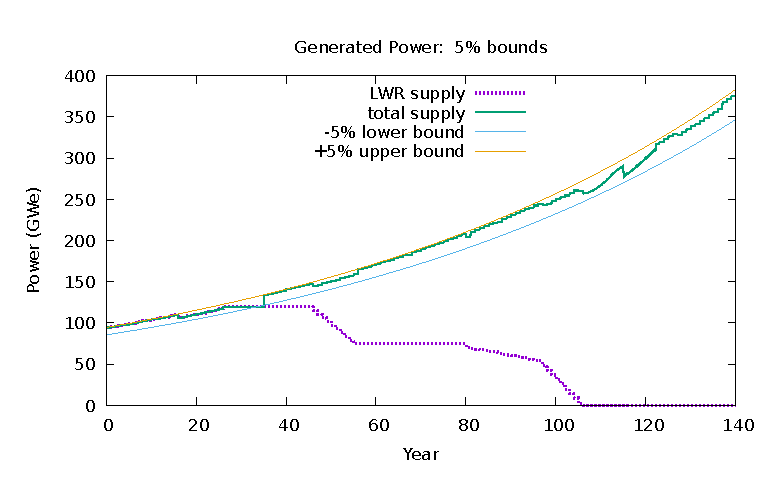
\includegraphics[width=1.0\textwidth]{best-known-power.eps}
    \caption[Power for best build schedule with $\pm5\%$ bounds]{ Both
      \gls{LWR} and total (\gls{SFR} and \gls{LWR}) generated power over time
      for the best deployment schedule found by the PSwarm optimizer using
      smaller $\pm5\%$ bounds around the 1\% power growth curve and annual
      deployments.  }

    \label{fig:exp1-bestknownpower}
\end{figure}

\subsection{Disruption Analysis}
\subsubsection{Motivation}
\subsubsection{Problem Definition}
\paragraph{Characteristics of disruption}
\paragraph{Choice of objective function}
\subsubsection{Implementation}
\paragraph{Avoiding nested optimization}
\paragraph{}
